\subsection{expr}
\paragraph{Funktionalitet}
\emph{expr} är ett kommandotolkverktyg som utvärderar uttryck med tal, strängar och jämförelser. För att undvika att kommandotolken utvärderar uttrycken måste speciella karaktärer utflys med \\. 
\paragraph{Exempel: matematiskt uttryck}
\begin{center}
        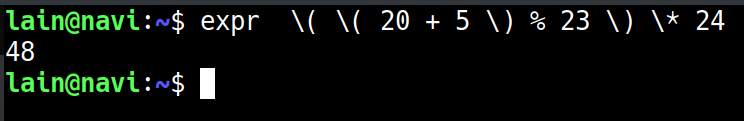
\includegraphics[width=\linewidth]{bilder/expr_matte.png}
        \captionof{figure}{Utvärdering av matematiskt uttryck}
\end{center}
I figuren demonstreras hur aritmetik och uträkningar kan utföras.
\paragraph{Exempel: blandat uttryck}
\begin{center}
        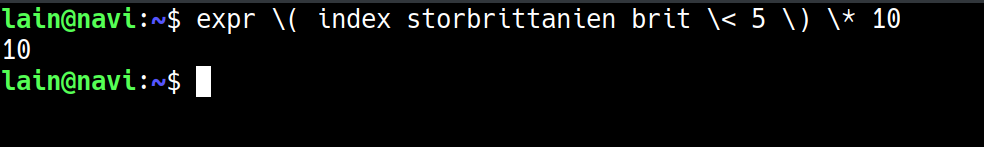
\includegraphics[width=\linewidth]{bilder/expr_blandat.png}
        \captionof{figure}{Utvärdering av blandat uttryck}
\end{center}
I exemplet utvärderas uttryck med både matematiska tal och karaktärer. Uttrycket mäter först vart i strängen "storbrittanien" som "brit" förekommer och jämför sedan om indexet är mindre än 5. Resultatet blir sant, en 1:a, vilket sedan multiplikeras med 10.  
\paragraph{Exempel: reguljära uttryck}
\begin{center}
        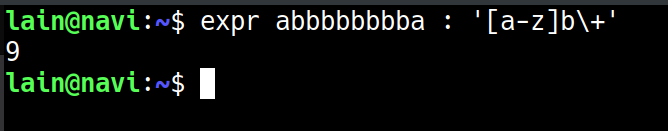
\includegraphics[width=\linewidth]{bilder/expr_regular.png}
        \captionof{figure}{Utvärdering av reguljärt uttryck}
\end{center}
I figuren visar ett reguljärt uttryck som räknar hur många gånger det förekommer bokstaven b en eller flera gånger med bokstäver från a-z framför.
